\documentclass{beamer}
\mode<presentation>{\usetheme{Frankfurt}}

\usepackage[english]{babel}
\usepackage[utf8]{inputenc}
\usepackage{times}
\usepackage[T1]{fontenc}

\usepackage{amsmath}
\usepackage[all]{xy}

\title{Text Surgery with vi}
\author{Nicholas C.~Spinale}
\institute{DevX \\ Carleton College}
\date{May 14^{th}, 2014}

\pgfdeclareimage[height=1cm]{thelogo}{images/devx-logo.png}
\logo{\pgfuseimage{thelogo}}

\AtBeginSubsection
    {
    \begin{frame}<beamer>{Outline}
        \tableofcontents[currentsubsection]
    \end{frame}
    }

\begin{document}

            \begin{frame}
            \titlepage
            \end{frame}

    \section*{Introduction}

            \begin{frame}{Introduction}
                \begin{center}
                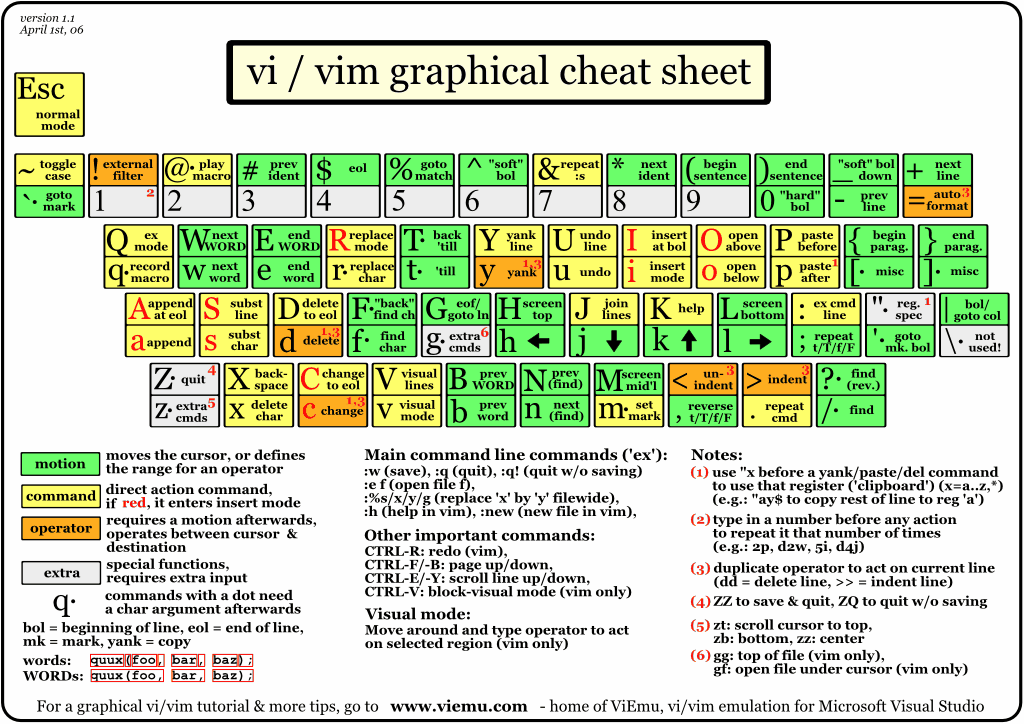
\includegraphics[width = 9.5cm, height = 7cm]{images/vi_vim_cheat_sheet.png}
                \end{center}
            \end{frame}

            \begin{frame}{My Plan}
            \tableofcontents
            \end{frame}

    \section{Background}

        \subsection{History}

            \begin{frame}{History}
                \begin{columns}[c]
                    \column{.5\textwidth}
                    Evolution of line editors
                    \begin{itemize}
                        \item 1971: ed at AT\&T
                        \item 1976: ex 0.1 by Bill Joy
                        \item 1979: ex 2.0/vi
                    \end{itemize}
                    \column{.4\textwidth}
                    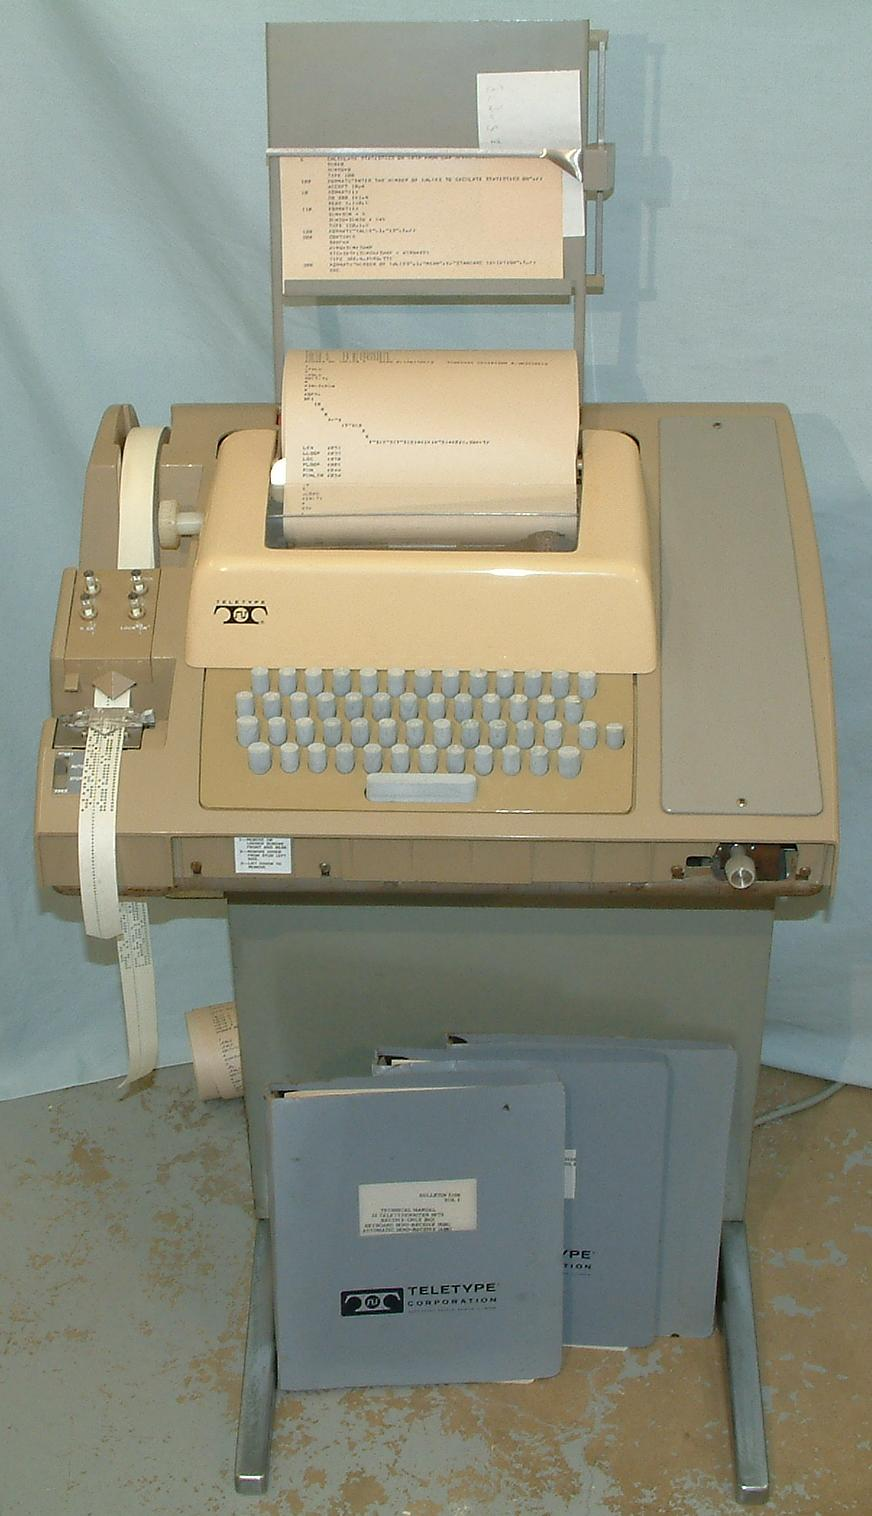
\includegraphics[height = 6cm]{images/teletype.jpg}
                \end{columns}
            \end{frame}

        \subsection{The vi Utility}

            \begin{frame}{The vi Utility}
                \texttt{vi [-rR] [-c command] [-t tagstring] [-w size] [file...]}
            \end{frame}

    \section{How to vi}

        \subsection{General Principles}

            \begin{frame}{wut is editor}
                \pause
                At the very least, it allows a user to
                \begin{itemize}
                    \pause
                    \item Load state of system into internal state
                    \pause
                    \item Modify internal state
                    \begin{itemize}
                        \pause
                        \item Buffers
                        \pause
                        \begin{itemize}
                            \item Contents
                            \item Position of cursor
                            \item Positions of other markers
                        \end{itemize}
                        \pause
                        \item Registers
                        \pause
                        \item Layout of buffers
                    \end{itemize}
                    \pause
                    \item Apply changes in internal state to system
                \end{itemize}
            \end{frame}

            \begin{frame}{A Clever Approach}
                Most editors: Key combinations \\~\\
                \pause
                vi: Modal editing/key sequences
            \end{frame}

        \subsection{Command Structure}

            \begin{frame}{Command Structure}
                \begin{center}
                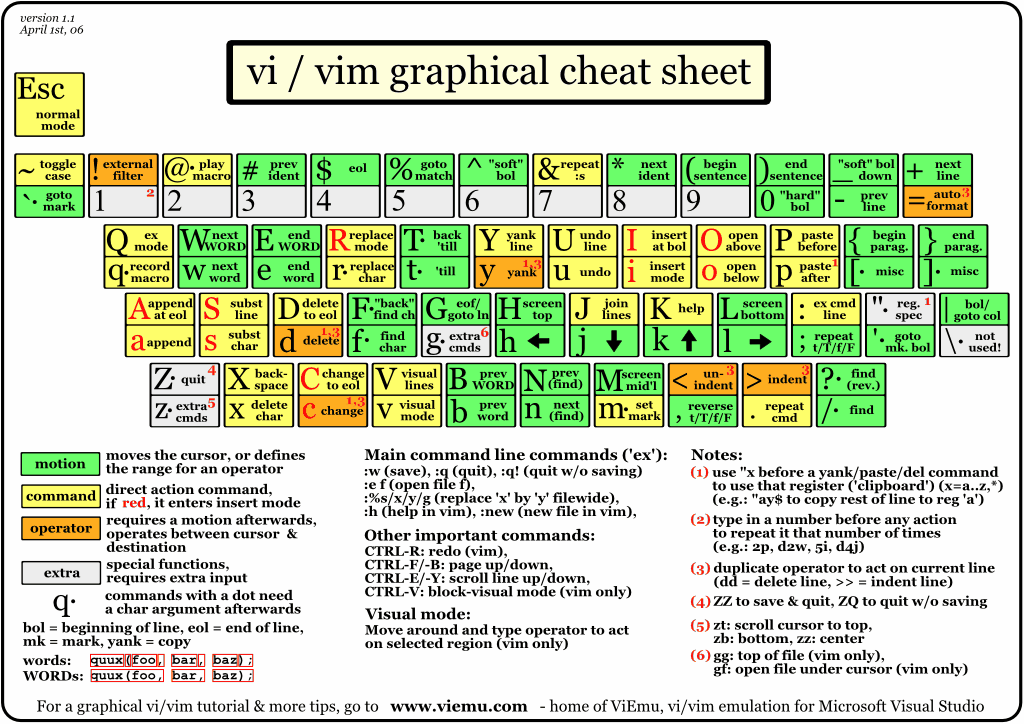
\includegraphics[width = 9.5cm, height = 7cm]{images/vi_vim_cheat_sheet.png}
                \end{center}
            \end{frame}

        \subsection{Registers}

            \begin{frame}{Registers}
                Named variables that store strings \\~\\
                Cut/copy to them \\
                Record them \\~\\
                Paste from them \\
                Play them
            \end{frame}

            \begin{frame}{The Art of Macros}
                Stay abstract. \pause Practice. \pause That is all.
            \end{frame}

            \begin{frame}{vi Golf}
                \texttt{i1<esc>qqyyp<c-a>q98@qqqcc Buzz<esc>5-q19@q2-qqciwFizz<esc>3+0q32@q}
            \end{frame}

    \section{Modern vi}

        \subsection{Vim}

            \begin{frame}{vi Improved}
                Ubiquitous \\~\\
                Compatability mode \\~\\
                Improvements
                \begin{itemize}
                    \item Aesthetics
                    \item Much more custmizability (including aesthetics...)
                    \item GUI mode
                \end{itemize}
            \end{frame}

            \begin{frame}{VimScript}
                There are TONS of plugins \\~\\
                Examples
                \begin{itemize}
                    \item Commentary
                    \item Tablizarize
                    \item Nerdtree
                    \item Ctrl-P
                \end{itemize}
            \end{frame}

        \subsection{Comparison to Other Editors}

            \begin{frame}{Emacs}
                \begin{center}
                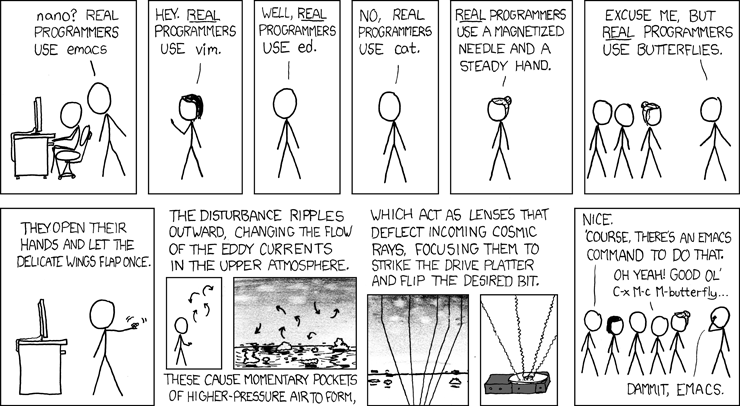
\includegraphics[width = 9.5cm, height = 5cm]{images/real_programmers.png}
                \end{center}
            \end{frame}

            \begin{frame}{IDE's}
                Pro: stay in terminal (seamlessly integrates with tmux, screen, etc) \\~\\
                \pause
                Con: learning curve
            \end{frame}

    \section*{Conclusion}

            \begin{frame}{Conclusion}
                \begin{center}
                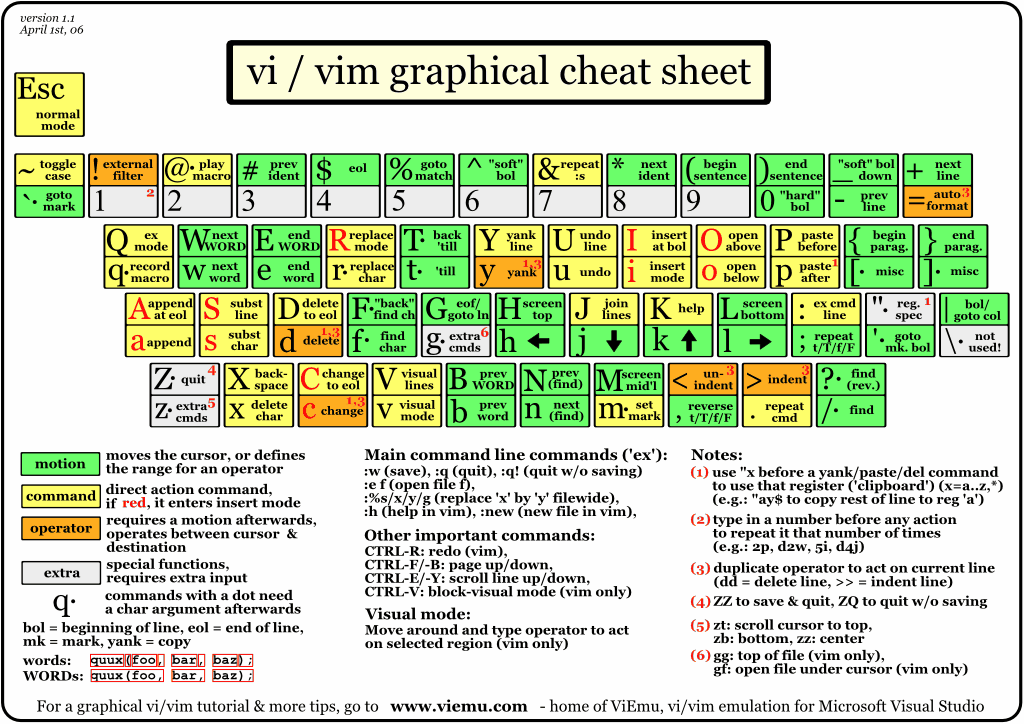
\includegraphics[width = 9.5cm, height = 7cm]{images/vi_vim_cheat_sheet.png}
                \end{center}
            \end{frame}


            \begin{frame}{Further Learning}
                How to continue learning
                \begin{itemize}
                    \item Cheatsheets (a few commands at a time)
                    \item VimDoc
                    \item VimCasts
                    \pause
                    \item Me \pause (I love talking about vim)
                \end{itemize}
            \end{frame}

            \begin{frame}{Questions?}
                \center{?}
            \end{frame}

\end{document}
